% TEXINPUTS=.:$HOME/git/bvtex: latexmk  -pdf <main>.tex
\documentclass[xcolor=dvipsnames]{beamer}

\input{defaults}
\input{beamer/preamble}

\setbeamertemplate{navigation symbols}{}
% \setbeamertemplate{background}[grid][step=1cm]

\usepackage{siunitx}
\usepackage{xmpmulti}
\usepackage[export]{adjustbox}
\usepackage{ulem}
\usepackage[outline]{contour}
\usepackage{tikz}
\usetikzlibrary{shapes.geometric, arrows}
\usetikzlibrary{positioning}

\definecolor{bvtitlecolor}{rgb}{0.98, 0.92, 0.84}
\definecolor{bvoutline}{rgb}{0.1, 0.1, 0.1}

\renewcommand{\bvtitleauthor}{Brett Viren}
\renewcommand{\bvtit}{LARF}
\renewcommand{\bvtitle}{\LARGE 3D Detector Response Calculations\\Using \textbf{B}oundary \textbf{E}lement \textbf{M}ethod}
\renewcommand{\bvevent}{DUNE Collab\\Sep 2016}
\renewcommand{\bvbeamerbackground}{}

\newcommand{\microboone}{MicroBooNE\xspace}

\def\Put(#1,#2)#3{\leavevmode\makebox(0,0){\put(#1,#2){#3}}}


\begin{document}
\input{beamer/title.tex}
\input{beamer/toc.tex}



\section{Motivation}

\begin{frame}
  \frametitle{Why Calculate Fields}
  Electrostatic and Shockley-Ramo ``weighting'' fields determine:
  \begin{itemize}
  \item the path and velocity of drifting electrons.
  \item the shape and intensity of induced signals.
    \begin{itemize}
    \item[$\rightarrow$] collection signals are induction signals.
    \end{itemize}
  \item how we best extract our signals.
  \item ultimately what our events look like.
  \end{itemize}
\end{frame}


\begin{frame}
  \frametitle{2D Field Calculations}
  \begin{columns}
    \begin{column}{0.5\textwidth}
      \begin{center}
        \includegraphics[width=\textwidth,page=5,clip,trim=0 0 0 5mm]{GarfieldSimulation-BoYu.pdf}

        Bo Yu using Garfield
      \end{center}
    \end{column}
    \begin{column}{0.5\textwidth}
      \begin{itemize}
      \item \textbf{F}inite \textbf{E}lement \textbf{M}ethod, high
        precision over limited 2D region.
      \item Reproduces major features, especially in the bulk volume.
      \item Relatively fast, allows exploring parameter space.
      \end{itemize}
    \end{column}
  \end{columns}

\end{frame}

\begin{frame}
  \frametitle{Why 3D?}
  \begin{itemize}
  \item MicroBooNE sees U-plane signal features explained by
    \textbf{long range inductance}
    \begin{itemize}\footnotesize
    \item[$\rightarrow$] although effects have already been largely
      reproduced using 2D fields out to $\pm10$ wires
    \end{itemize}
  \item See V-plane signal features likely explained by 3D wire
    structure.
  \item Novel wire readout schemes have been proposed which are more
    sensitive to 3D crossing patterns.
  \item Detector edge effects are inherently 3D.
  \end{itemize}
\end{frame}

\begin{frame}
  \frametitle{Why BEM?}
  \textbf{B}oundary \textbf{E}lement \textbf{M}ethod
  \begin{itemize}
  \item FEM scales as the volume, BEM as the surface.
  \item BEM solution and evaluation decoupled, can evaluate at
    arbitrary points.
  \item BEM requires less CPU than FEM (hours vs days).
  \item BEM has less mature tools, so requires some development and
    validation for a given geometry.
  \end{itemize}
\end{frame}

\section{Procedure}

\begin{frame}
  \frametitle{Procedure Overview}
  \begin{enumerate}
  \item Define \textbf{wire geometry}
  \item Generate \textbf{surface mesh} on wires and drift voltage electrodes
  \item Solve \textbf{surface boundary conditions} for each field
    \begin{itemize}
    \item [$\rightarrow$] fields: \textbf{drift} and one \textbf{weighting}/wire
    \end{itemize}
  \item Define electron drift path \textbf{starting points}
  \item Step through \textbf{drift field} to produce \textbf{drift paths}.
  \item Sample \textbf{weighting field} for a given wire, along a path
    to produce corresponding \textbf{current waveform}.
  \item Define an average over paths to produce a \textbf{response
      function} for a given wire as a function of path location.
  \end{enumerate}
  Also: sample full-volume raster of field for debugging.
\end{frame}

\begin{frame}
  \frametitle{Wire Geometry}
  \begin{columns}
    \begin{column}{0.5\textwidth}
      \begin{center}
        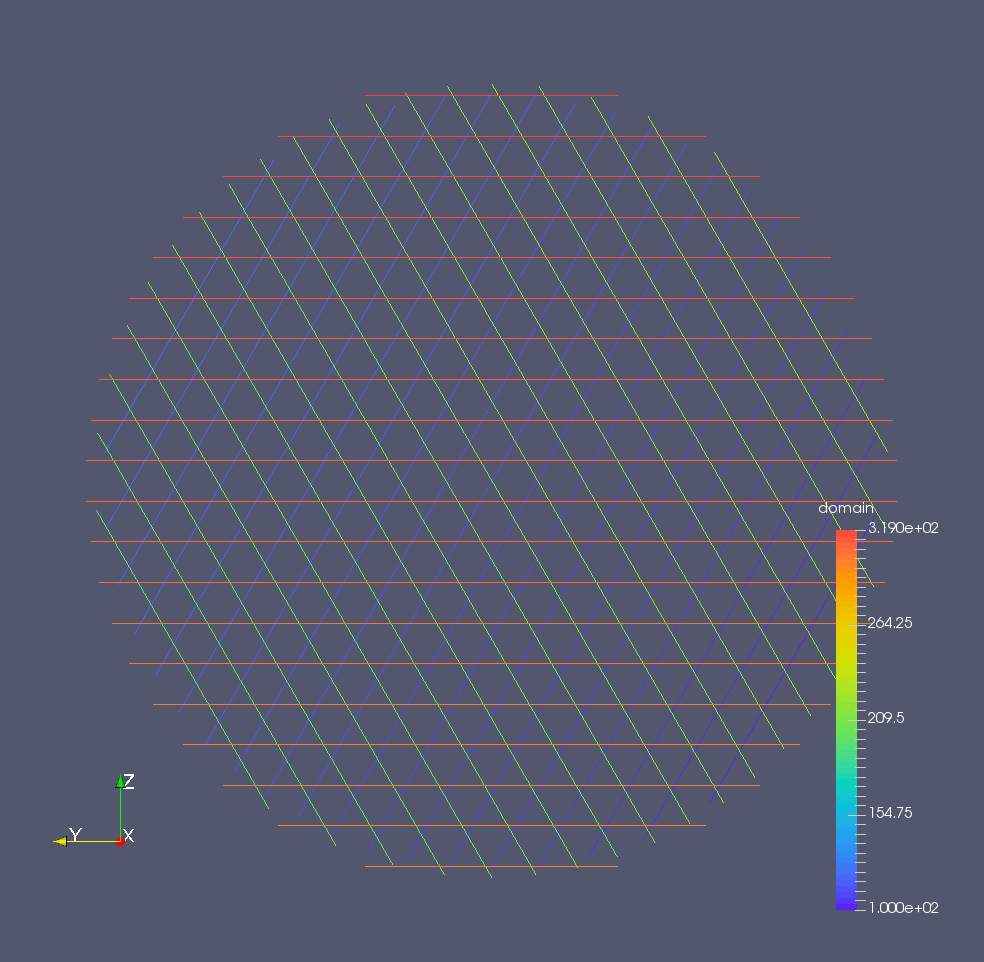
\includegraphics[width=\textwidth,clip,trim=2cm 1cm 2cm 2cm]{steps/wires1.png}
        
        $\mu$Boone-like, color is wire index
      \end{center}
    \end{column}
    \begin{column}{0.5\textwidth}
      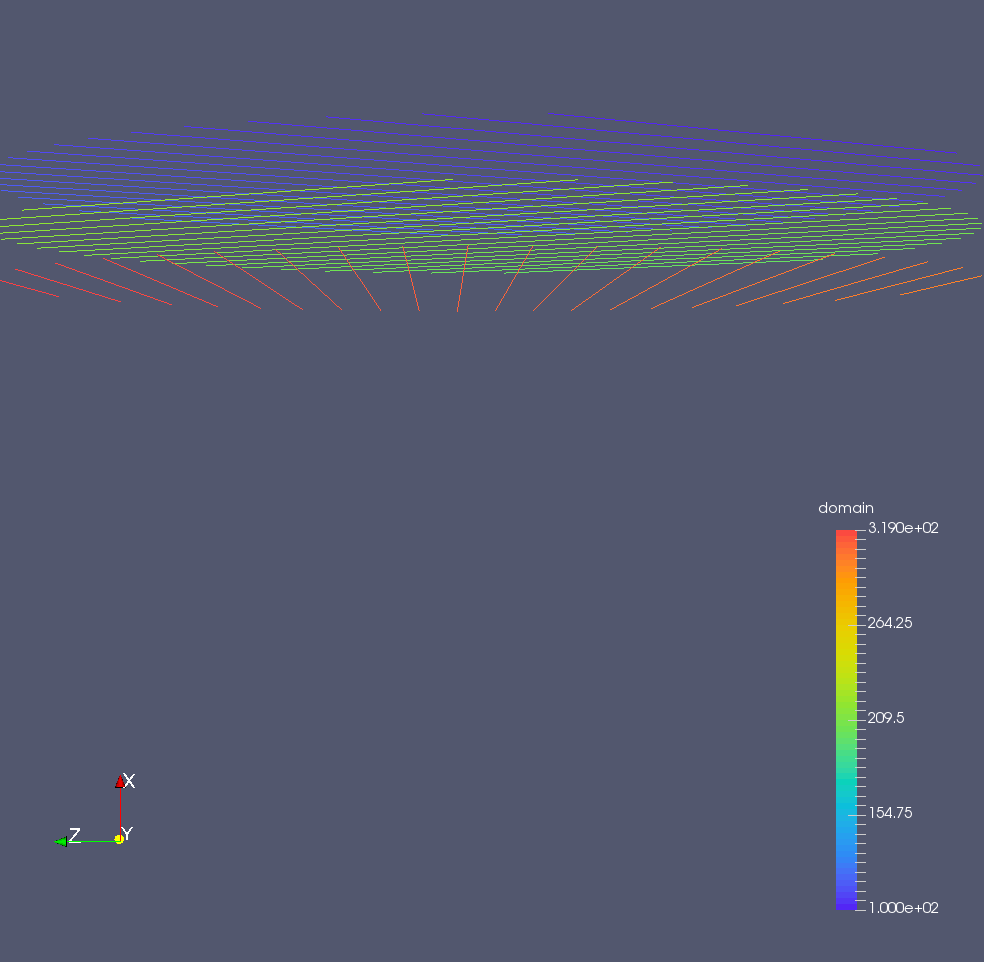
\includegraphics[width=\textwidth,clip,trim=0 22cm 0 2cm]{steps/wires2.png}
      
        \footnotesize
      \begin{itemize}
      \item Wires specified by their endpoints and a radius, 
        different wire envelopes possible.
      \item Parameterized wire generator included, covers DUNE, $\mu$Boone,
        others.
      \item Wires geometry seeds surface mesh and to govern
        electron/wire ``hits'' to stop path stepping.
      \item Wire extent drives scale (CPU/RAM) of calculation.
      \end{itemize}
    \end{column}
  \end{columns}

\end{frame}
\begin{frame}
  \frametitle{Surface Mesh}
  \begin{center}
    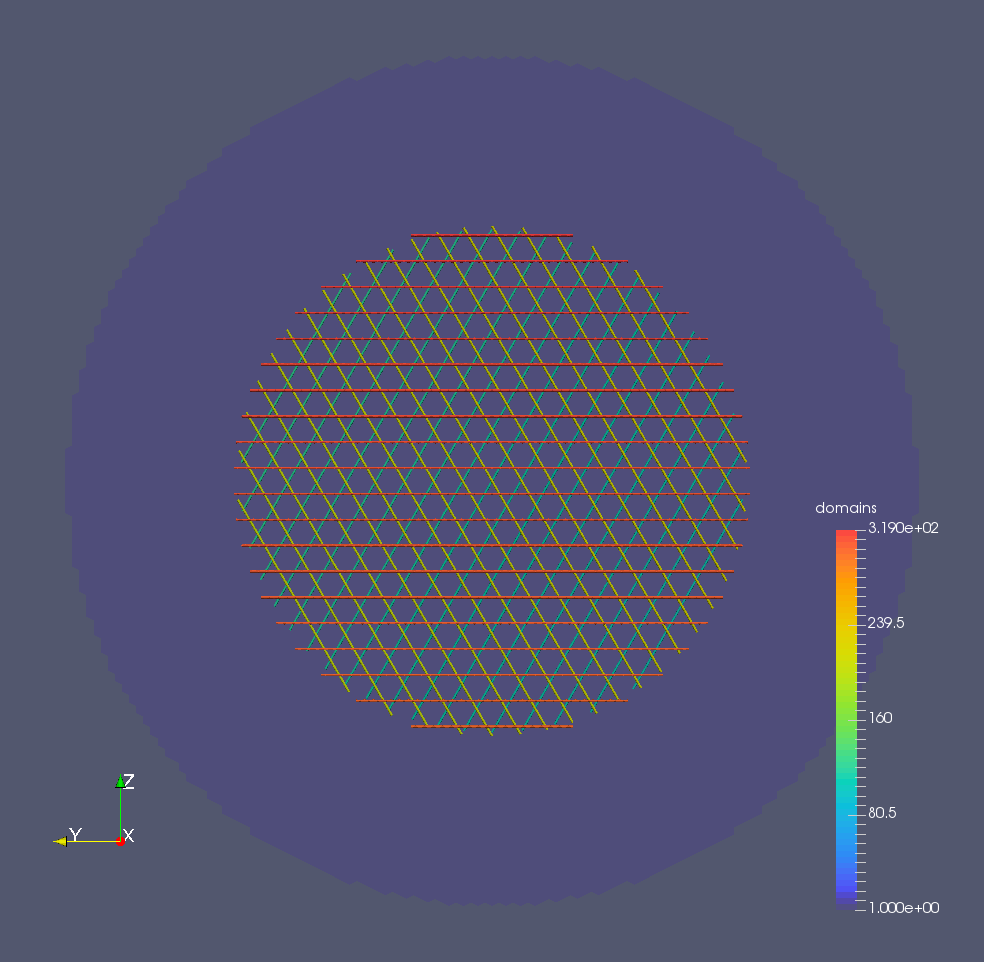
\includegraphics[height=5.5cm,clip,trim=0cm 0cm 0cm 0cm]{steps/surface1.png}%        
    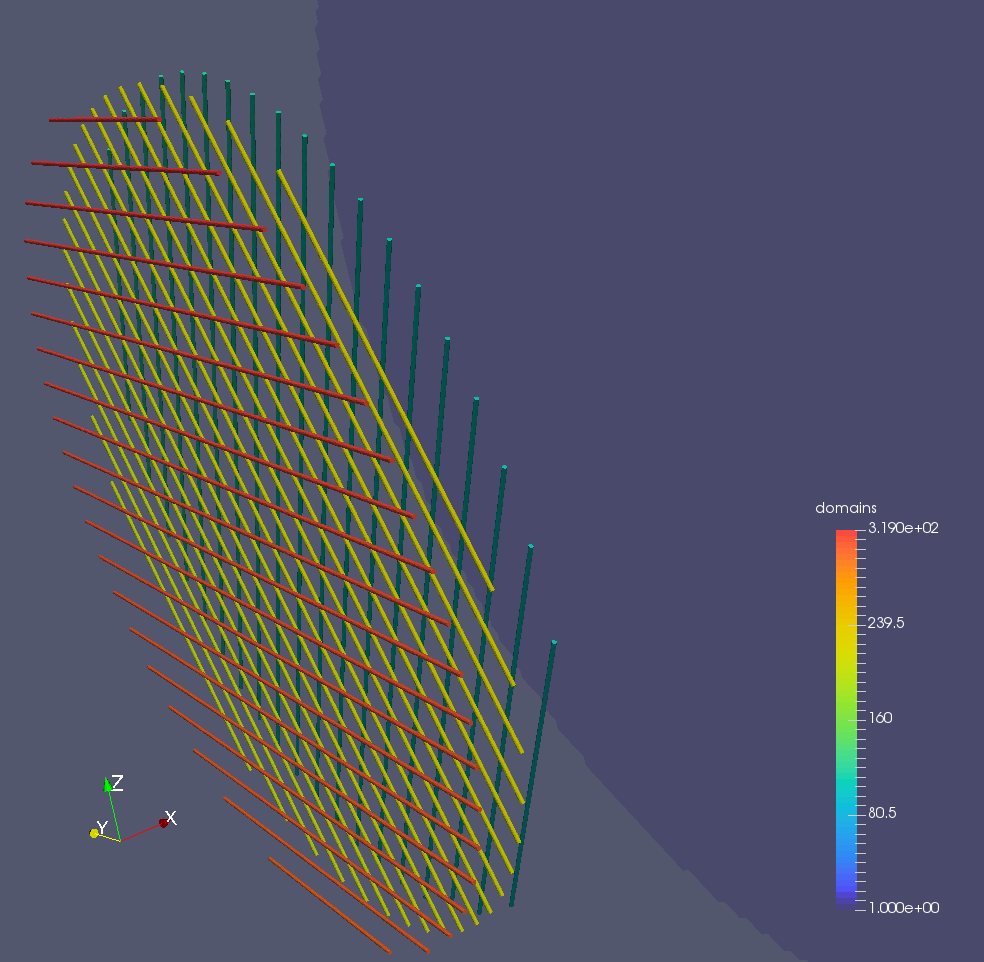
\includegraphics[height=5.5cm,clip,trim=0cm 0cm 10cm 0cm]{steps/surface3.png}

    \Put(100,350){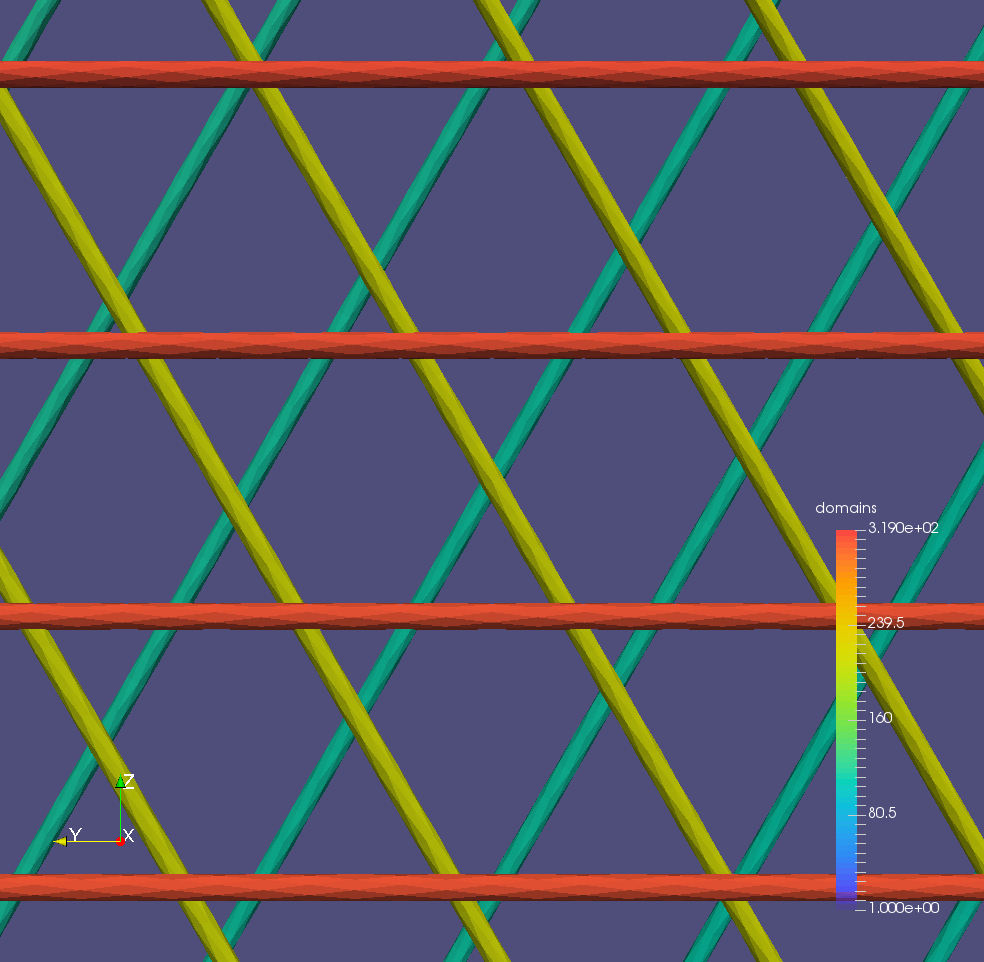
\includegraphics[height=2cm,clip,trim=0cm 0cm 0cm 0cm]{steps/surface2.png}}
  \end{center}
  \begin{itemize}
  \item Meshing of cylinders and flat disks provided.
    \begin{itemize}\footnotesize
    \item Can use GMSH or roll-your-own.
    \end{itemize}
  \item Mesh size drives determines accuracy (and run time).
  \end{itemize}

\end{frame}
\begin{frame}
  \frametitle{Boundary Conditions}
  \begin{center}
    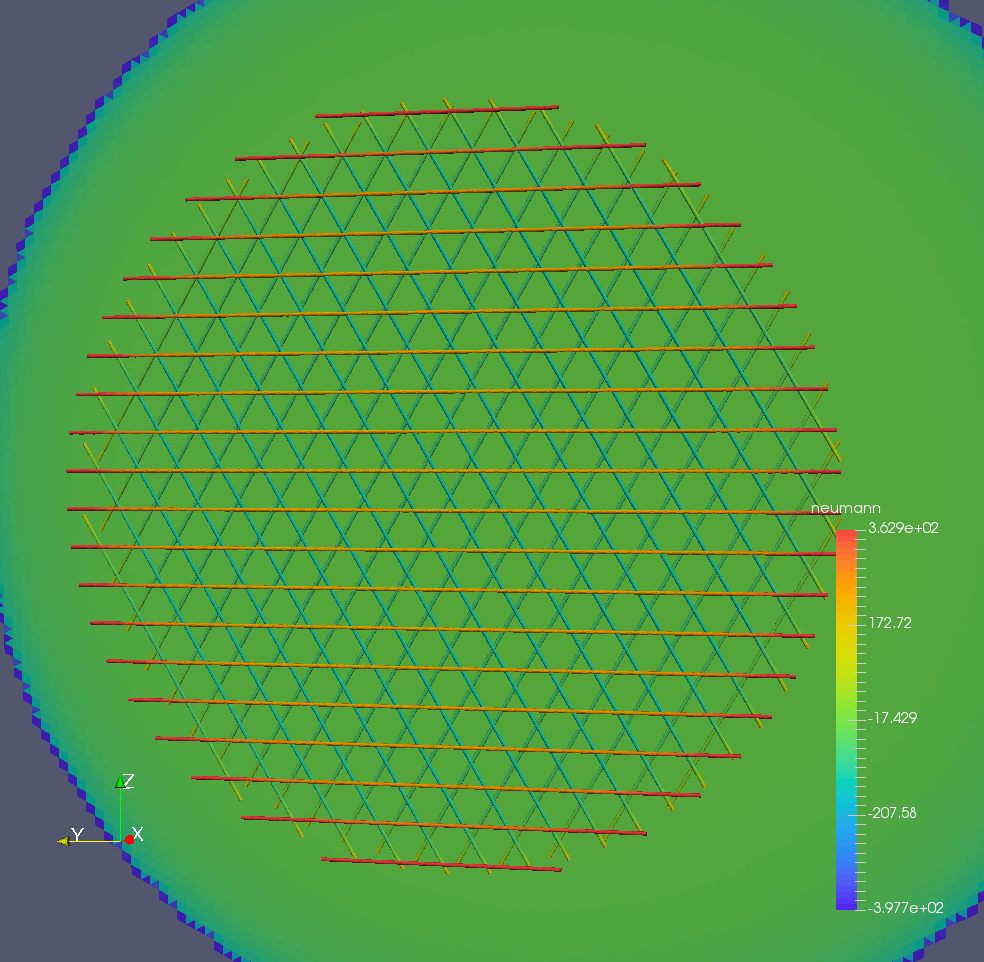
\includegraphics[height=5cm,clip,trim=0cm 0cm 0cm 0cm]{steps/drift-boundary1.png}%        
    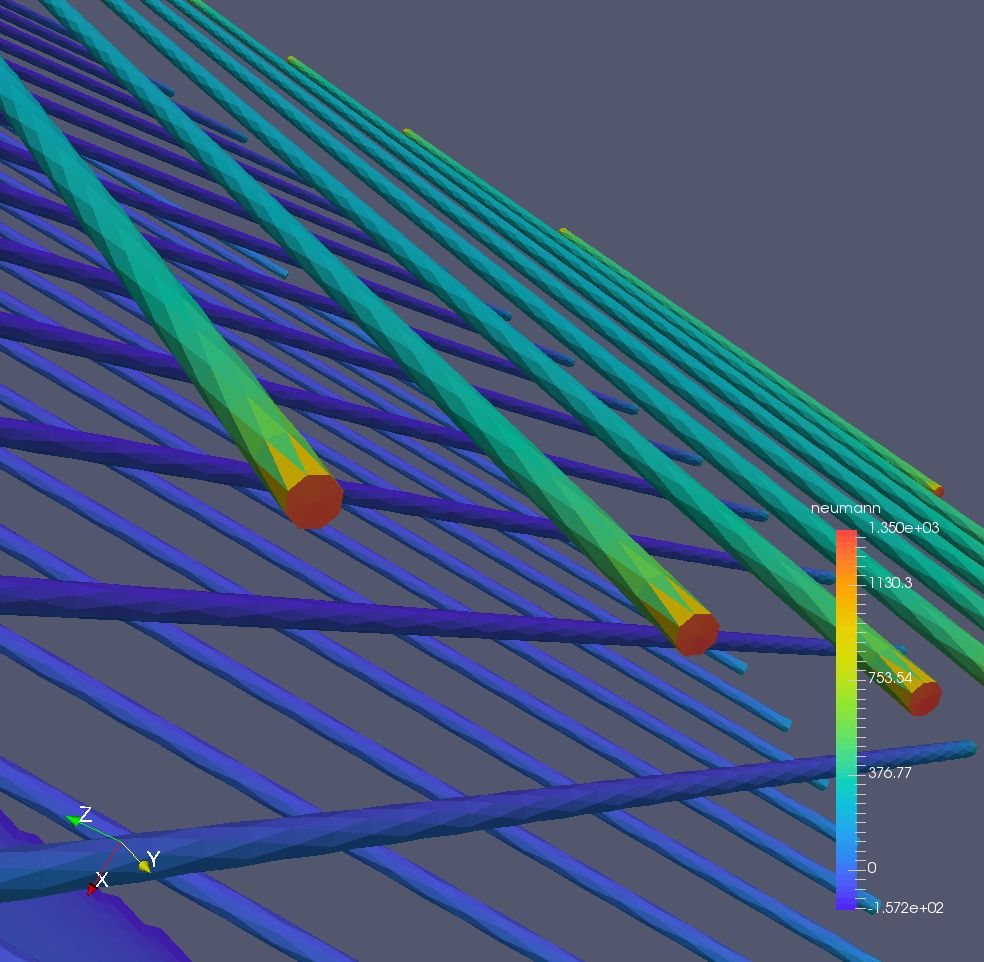
\includegraphics[height=5cm,clip,trim=0cm 0cm 00cm 0cm]{steps/drift-boundary2.png}

    \scriptsize Color is magnitude of E-field normal to surface.
    Note, scaled to show edge effects.
  \end{center}
  \begin{itemize}\footnotesize
  \item Apply scalar potential (Dirichlet) boundary conditions.
  \item BEM solves for \texttt{mag(norm(Efield)} (Neumann) boundary conditions.
  \item Finite sized geometry leads to unwanted edge effects.
  \end{itemize}
  
\end{frame}
\begin{frame}
  \frametitle{Starting Points}
  \begin{center}
    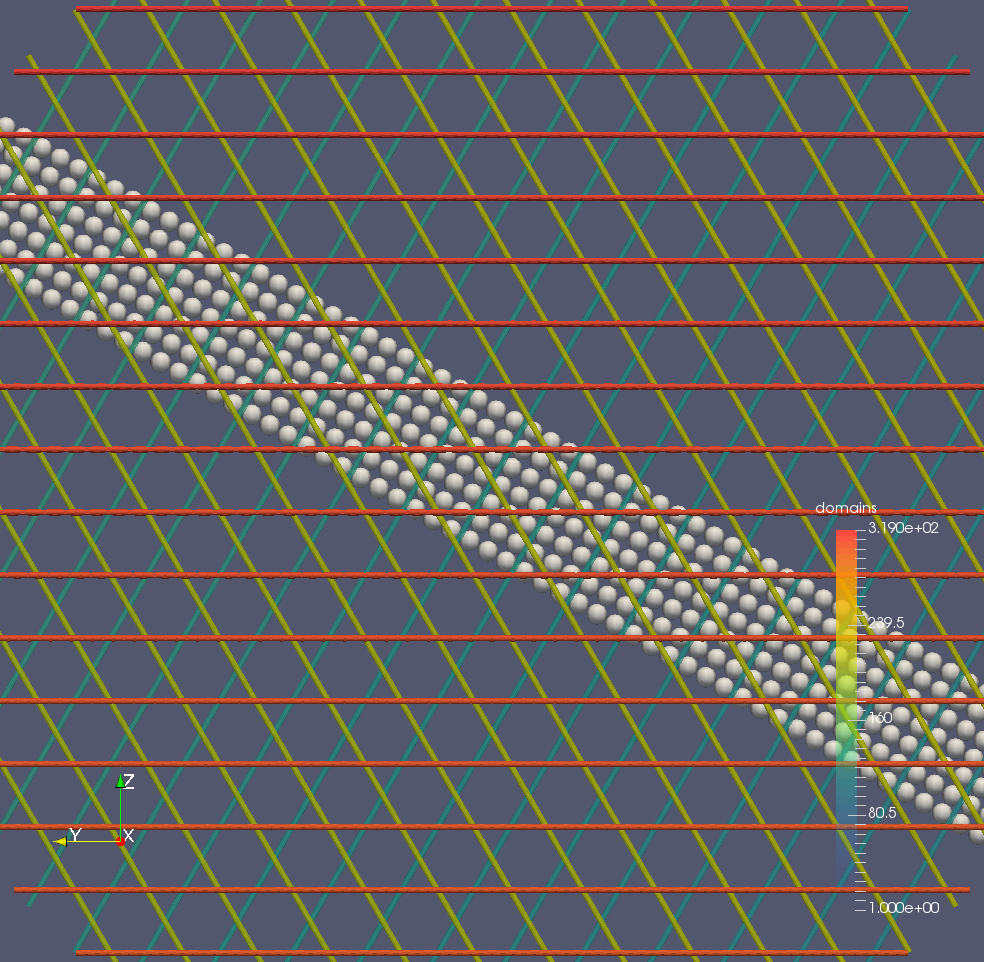
\includegraphics[height=5cm,clip,trim=0cm 0cm 0cm 0cm]{steps/ustarts1.png}%        
    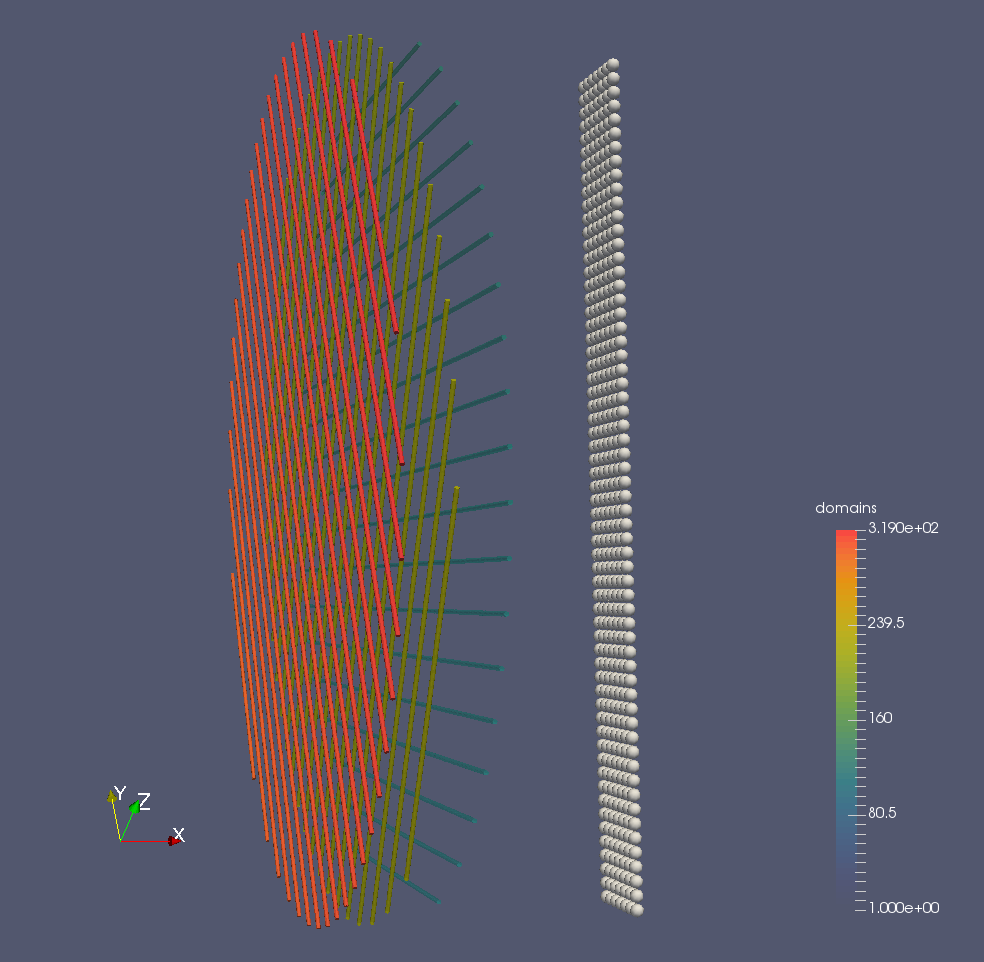
\includegraphics[height=5cm,clip,trim=0cm 0cm 00cm 0cm]{steps/ustarts2.png}
  \end{center}
  \begin{itemize}
  \item Generate starting points for drift paths.  
  \item Various schemes, this one aligns with wire-of-interest.
  \end{itemize}
  
\end{frame}
\begin{frame}
  \frametitle{Drift Path Views}
  \begin{center}
    
  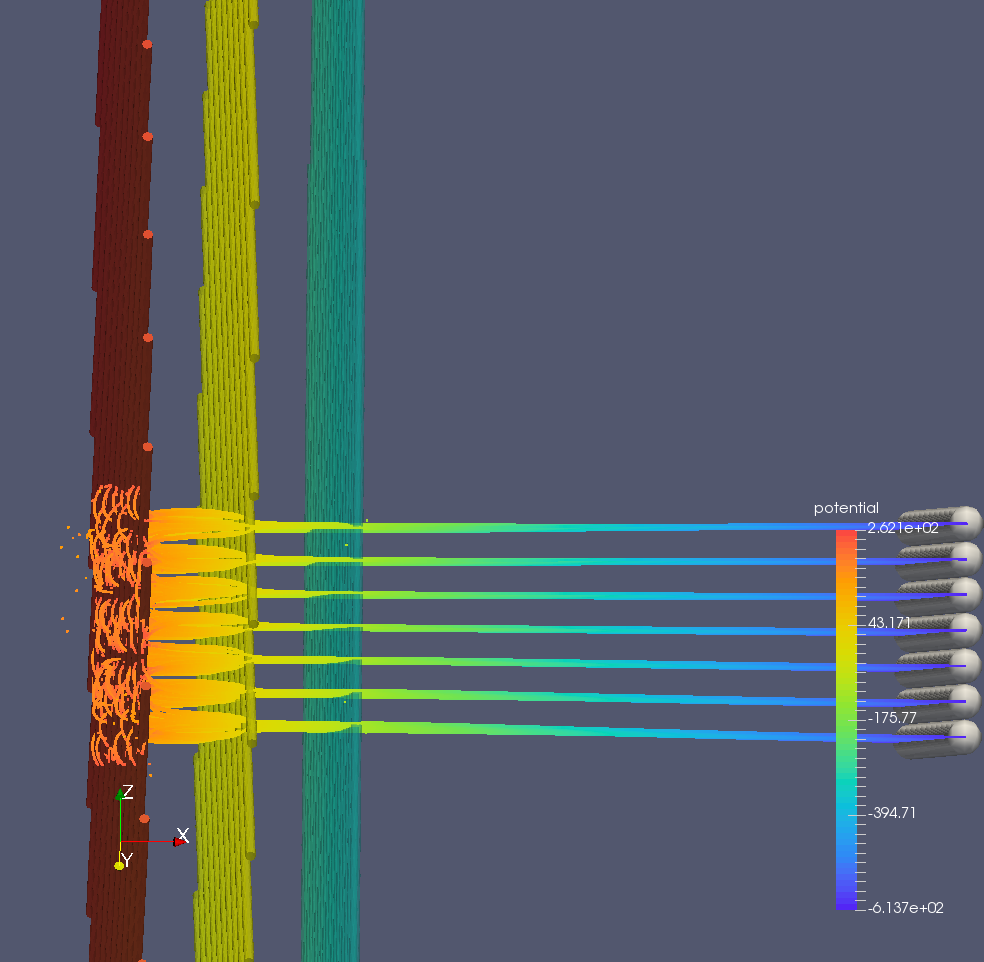
\includegraphics[height=3cm,clip,trim=0cm 5cm 0cm 17cm]{steps/upaths1.png}

  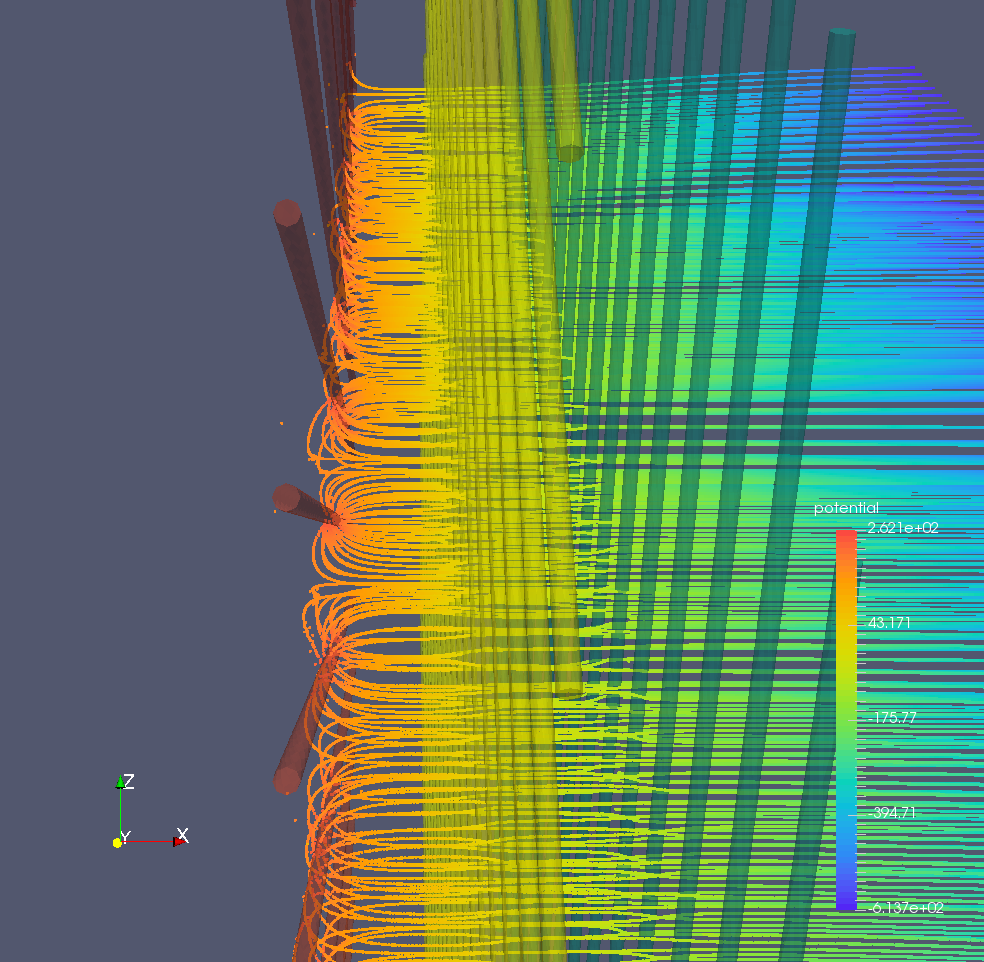
\includegraphics[height=4cm,clip,trim=10cm 0cm 10cm 0cm]{steps/upaths8.png}
  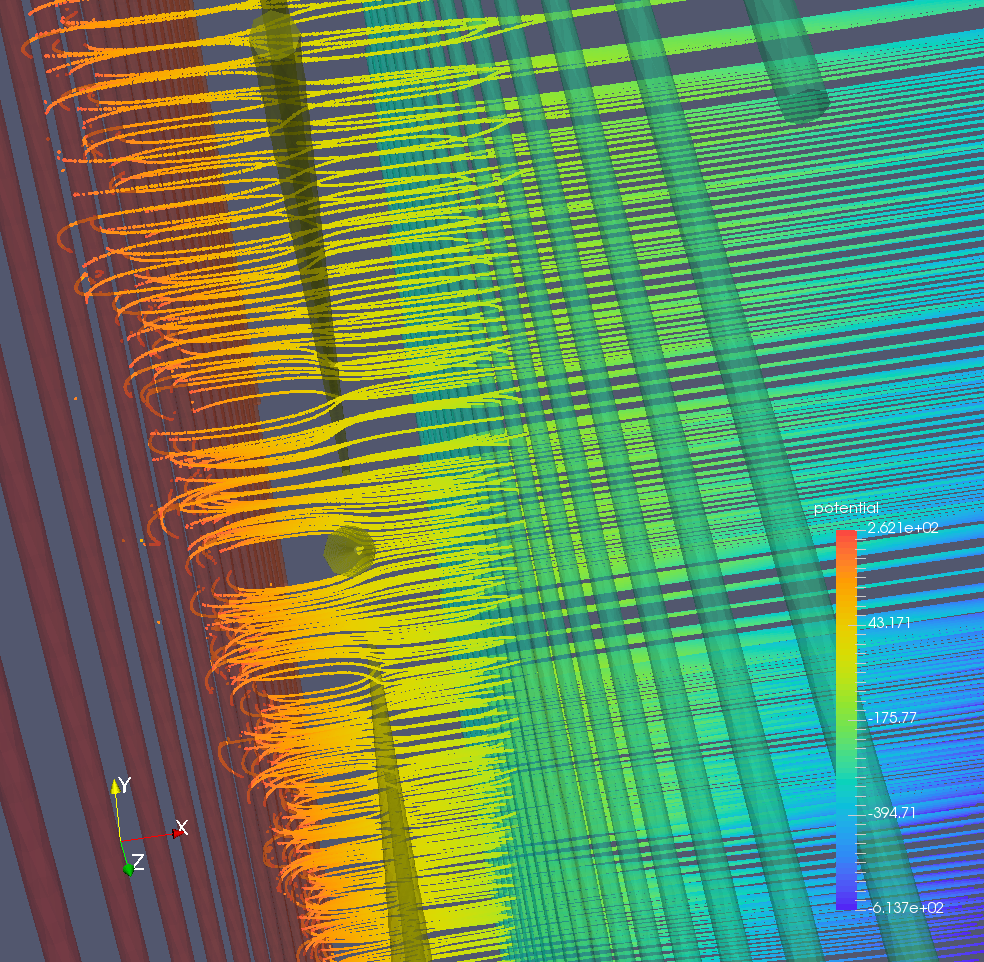
\includegraphics[height=4cm,clip,trim=4cm 0cm 10cm 0cm]{steps/upaths7.png}
  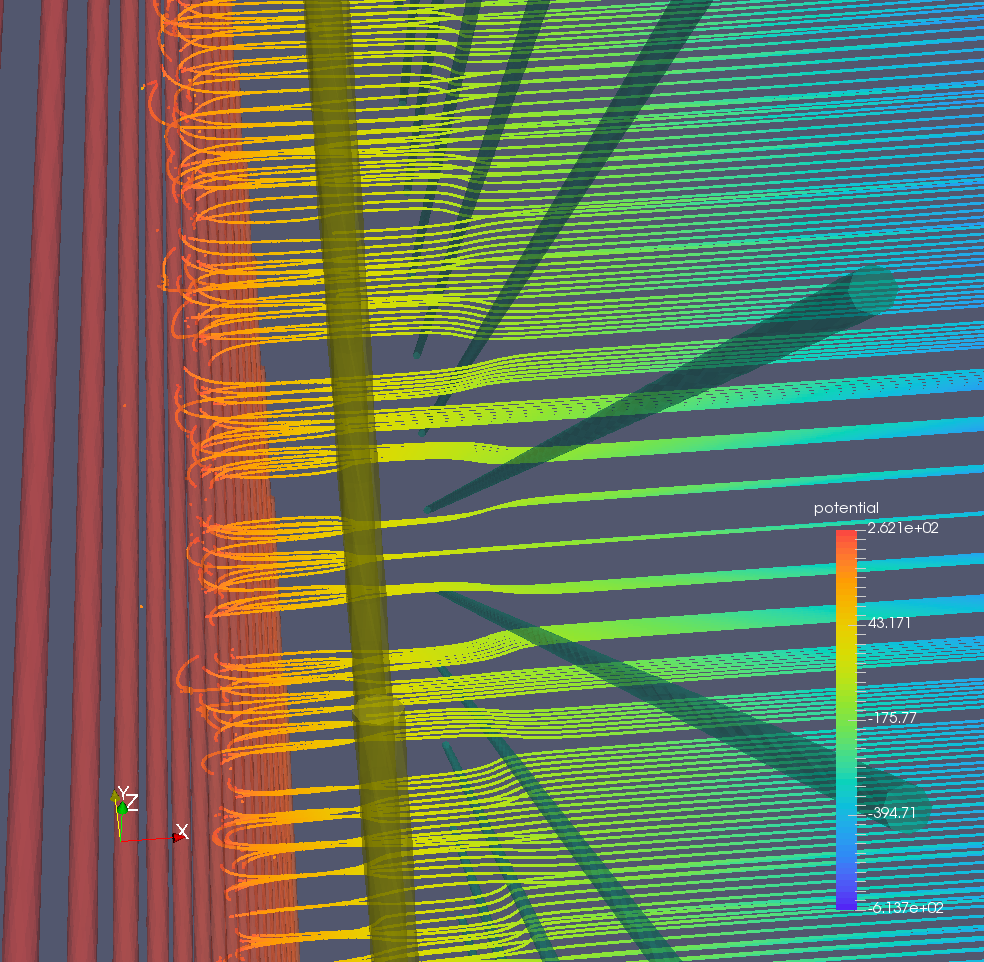
\includegraphics[height=4cm,clip,trim=4cm 0cm 10cm 0cm]{steps/upaths6.png}
  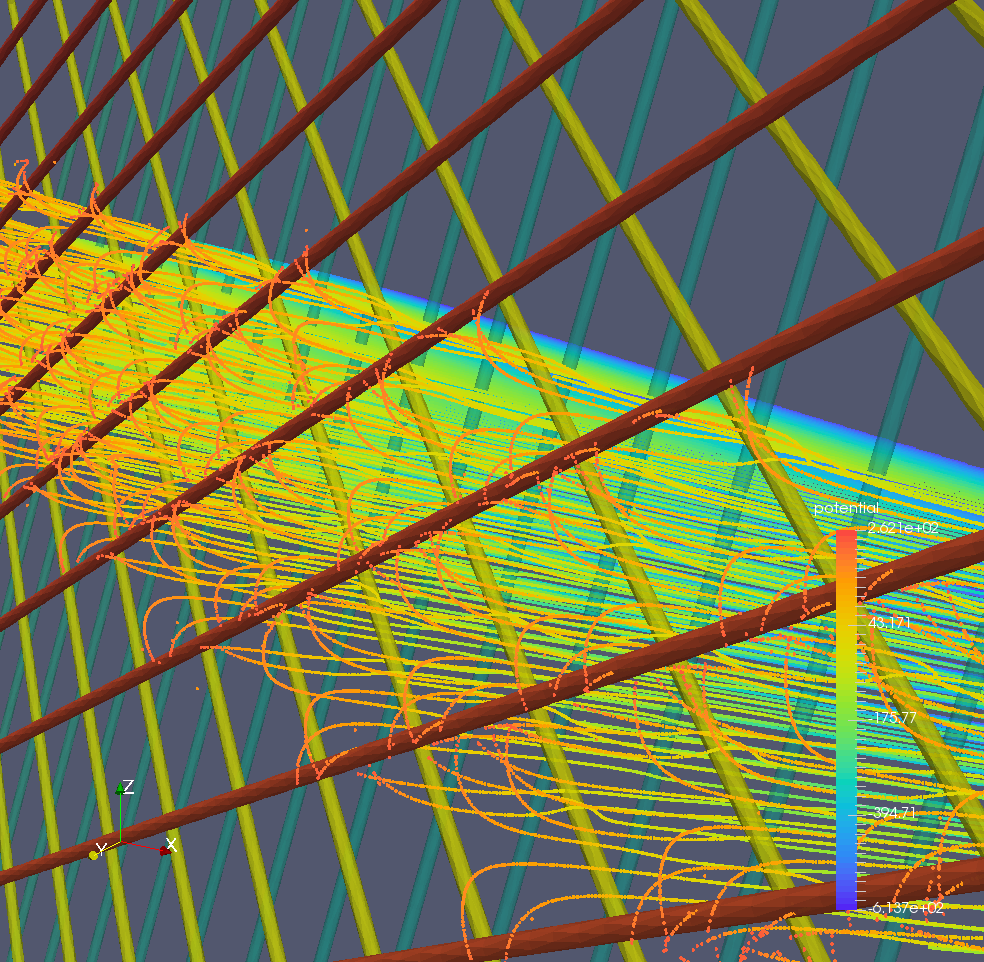
\includegraphics[height=4cm,clip,trim=10cm 0cm 0cm 10cm]{steps/upaths5.png}
  \end{center}


\end{frame}
\begin{frame}
  \frametitle{Stepping to Produce Paths}
  \begin{center}
    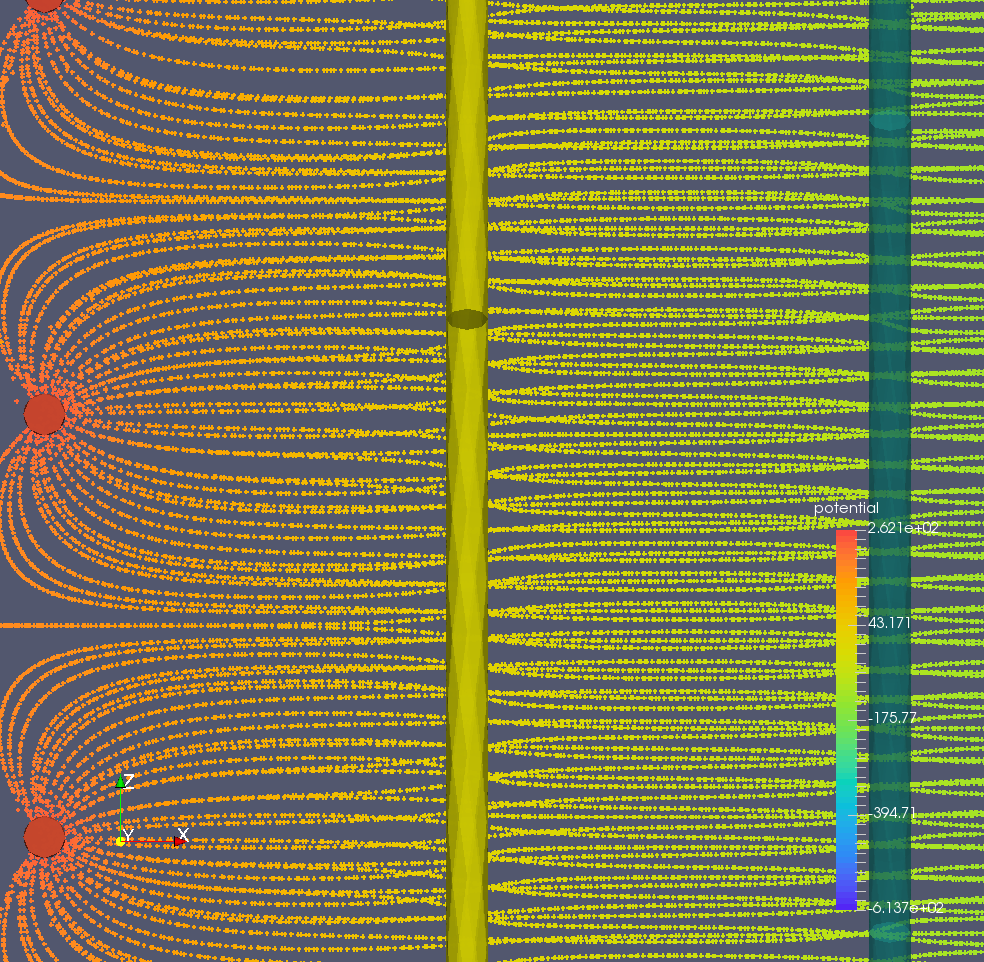
\includegraphics[height=5cm,clip,trim=0cm 0cm 0cm 17cm]{steps/upaths3.png}
    % 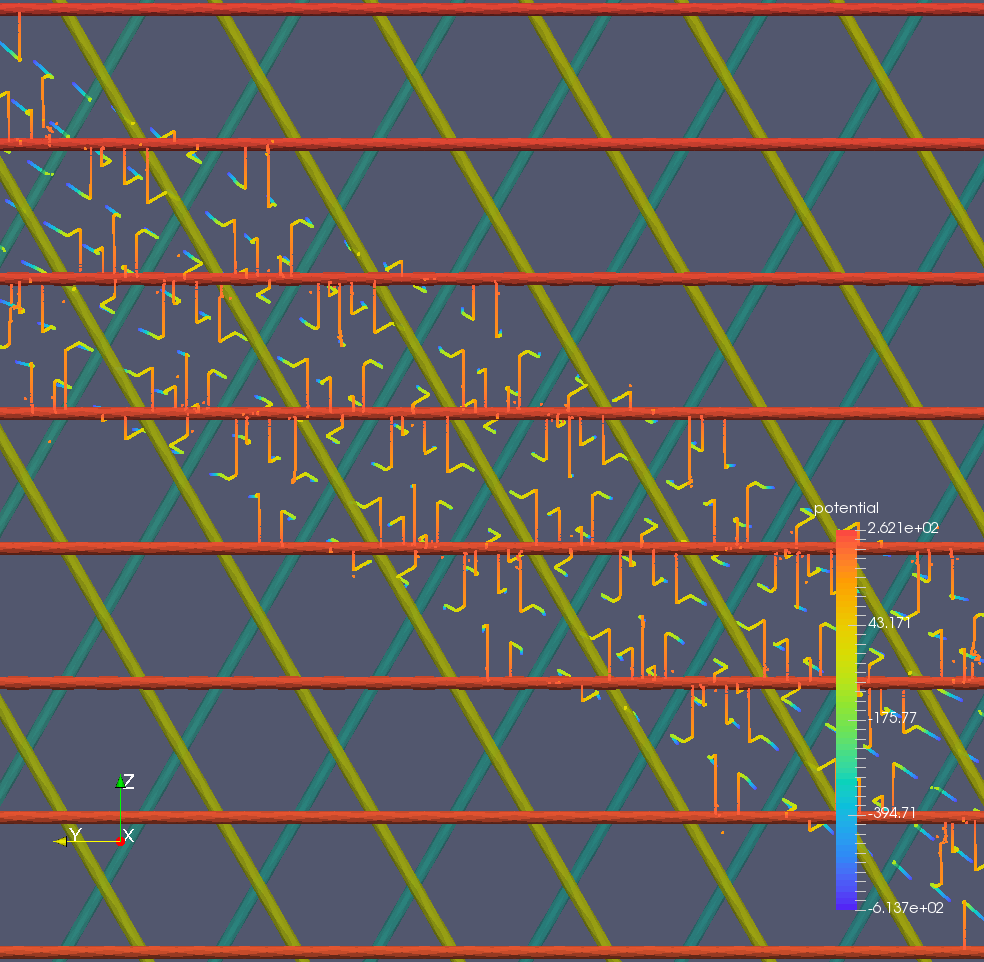
\includegraphics[height=3cm,clip,trim=0cm 10cm 0cm 10cm]{steps/upaths4.png}
  \end{center}
  \begin{itemize}\footnotesize
  \item Steps use 5th order Runge-Kutta with fixed step size.
  \item Each sub-step evaluates potential on 7 points to get gradient.
  \item Steps terminate if they ``hit'' a wire.
  \end{itemize}

\end{frame}

\begin{frame}
  \frametitle{Edge Effects from Finite Geometry}
  \begin{columns}
    \begin{column}{0.4\textwidth}
      \begin{center}
        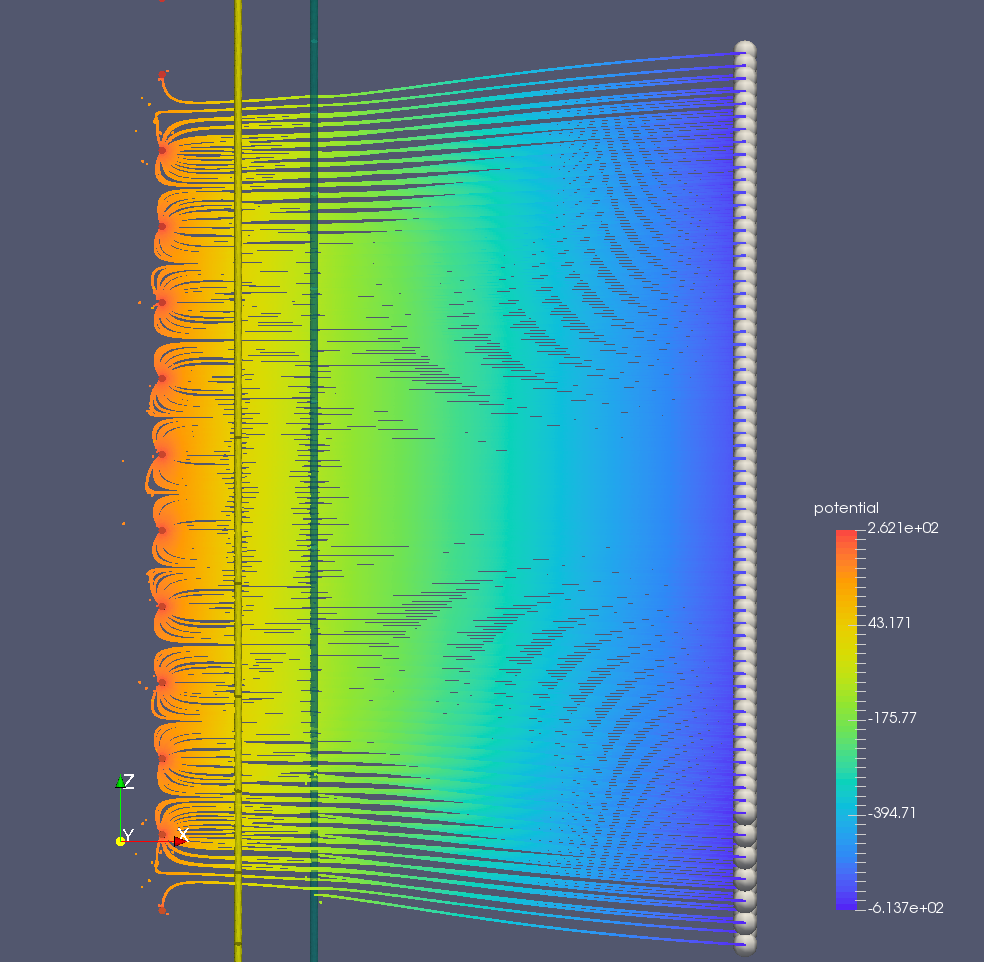
\includegraphics[width=\textwidth,clip,trim=4cm 0cm 10cm 0cm]{steps/upaths2.png}    
      \end{center}
    \end{column}
    \begin{column}{0.6\textwidth}
      \begin{itemize}
      \item Finite size ``cathode'' and wire planes lead to
        non-uniform fields near edge.
        \begin{itemize}\footnotesize
        \item Drift fields ``pinch in'' toward W-wires.
        \end{itemize}
      \item Need to explore ways to shape field.  Some possibilities:
        \begin{itemize}\footnotesize
        \item Smaller ``cathode'' disk?
        \item Larger ``cathode'' disk with a grounded annulus disk at X=0?
        \item Coaxial rings along X-axis with stepped voltage?
        \end{itemize}
      \item For now, live with small error.  
        \begin{itemize}\footnotesize
        \item Charge drifting near edge contributes $\ll 1$\%
        \end{itemize}
      \end{itemize}
    \end{column}
  \end{columns}
  
\end{frame}

\begin{frame}
  \frametitle{Weighting Field for U-wire}

  \footnotesize
  \begin{columns}
    \begin{column}{0.5\textwidth}
      \begin{center}
        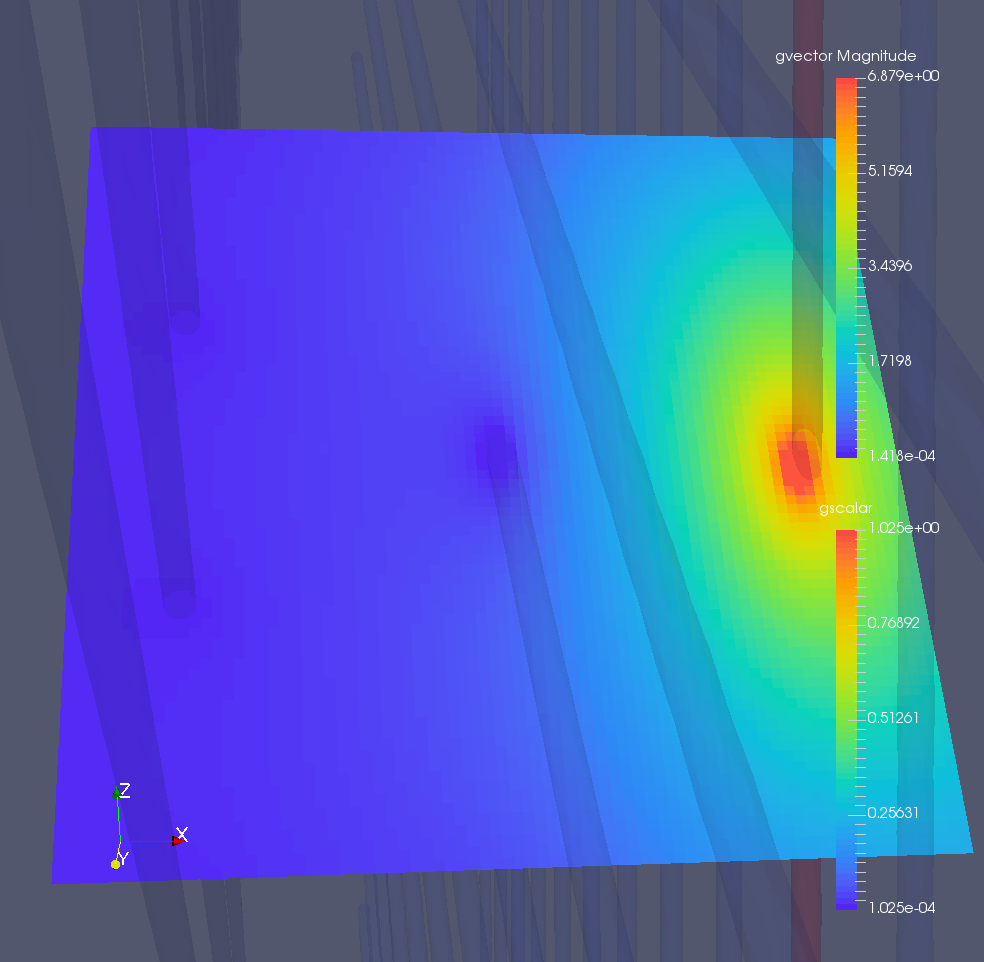
\includegraphics[width=0.9\textwidth,clip,trim=0cm 0cm 0cm 0cm]{steps/uweight4.png}
        
        Weighting \textbf{potential}.
      \end{center}      
    \end{column}
    \begin{column}{0.5\textwidth}
      \begin{center}
        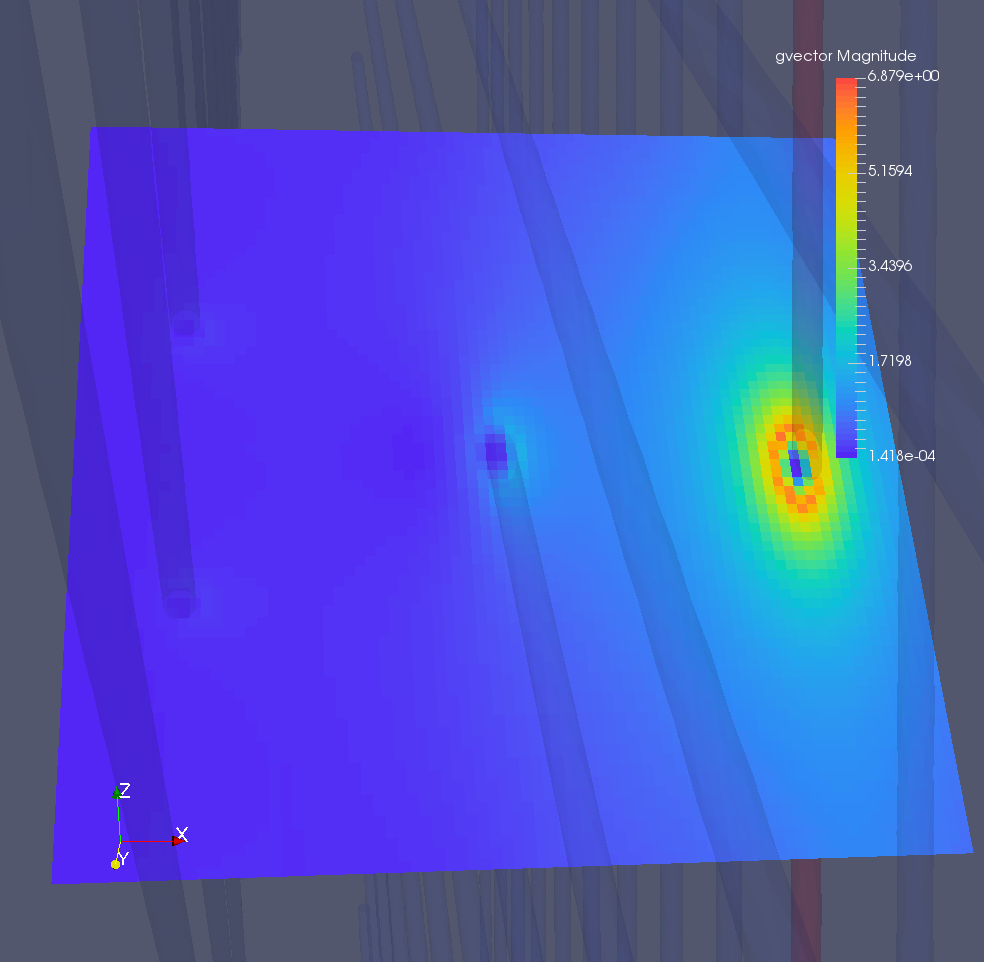
\includegraphics[width=0.9\textwidth,clip,trim=0cm 0cm 0cm 0cm]{steps/uweight2.png}%
        
        Weighting \textbf{gradient magnitude}.
      \end{center}      
    \end{column}
  \end{columns}
  \begin{center}
    Zoomed in to inter-plane region.
  \end{center}
\end{frame}


\begin{frame}
  \frametitle{Current Waveforms as Volumetric Data}
  \begin{center}
    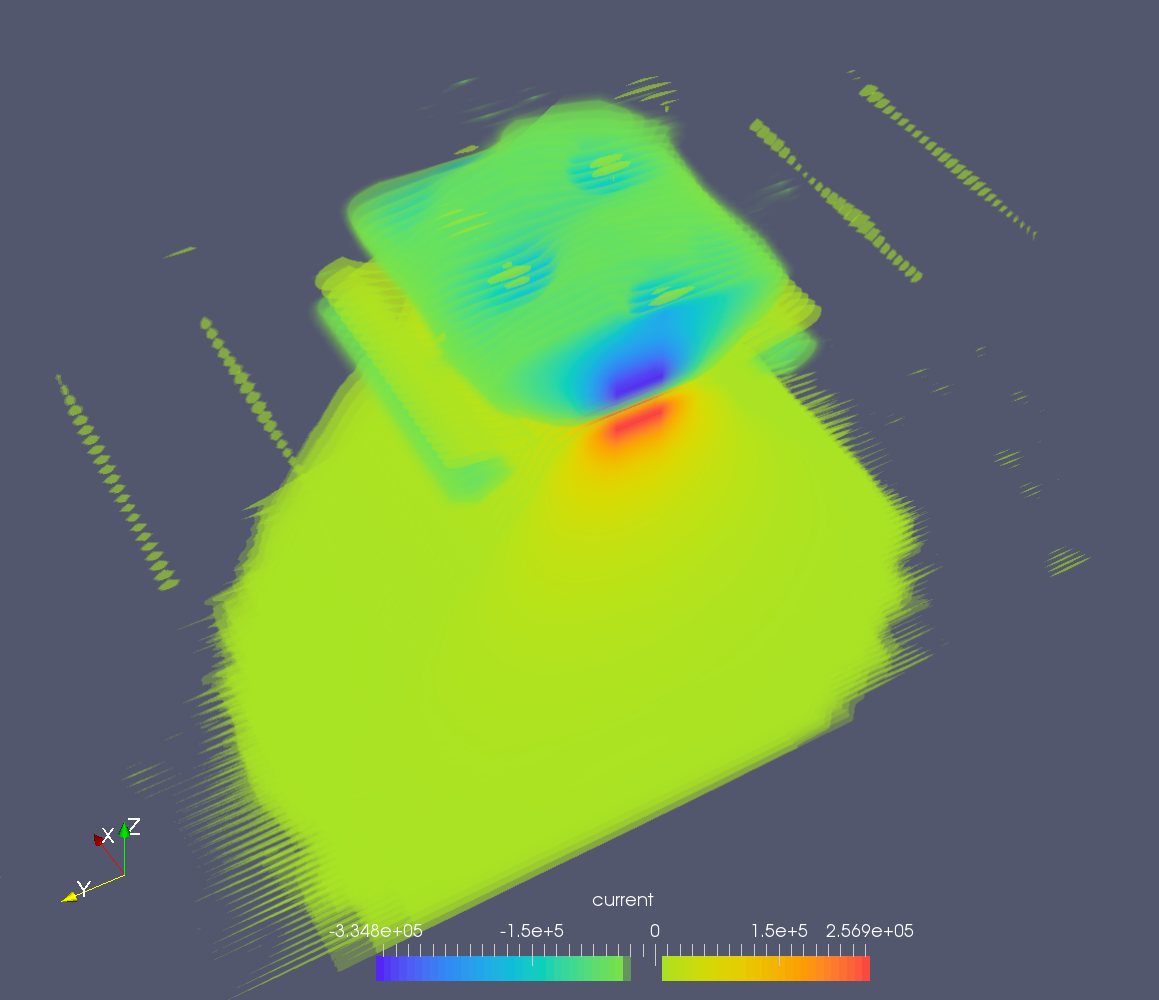
\includegraphics[height=7cm,clip,trim=0cm 0cm 0cm 0cm]{current-iso.png}

    \footnotesize
    X=along U-wire, Y=transverse to U-wire, Z=time, color=current.
  \end{center}

\end{frame}

\begin{frame}
  \frametitle{Current Waveforms vs. Transverse Location}
  \begin{center}
    Current (\textcolor{red}{red=positive}, \textcolor{blue}{blue=negative}, \textcolor{green}{green near zero}) \\
    in time vs position transverse to U-wire.

    \includegraphics<1>[height=5cm,clip,trim=0cm 8cm 0cm 8cm]{current-slice.png}
    \includegraphics<2>[height=5cm,clip,trim=0cm 8cm 0cm 8cm]{current-3d.png}
    
    \only<1>{One slice shows \textbf{spurious artifacts}.}
    \only<2>{Average over longitudinal lines of paths.}
  \end{center}
  
\end{frame}

\begin{frame}
  \frametitle{Response Functions - U Wire}
  \begin{center}
    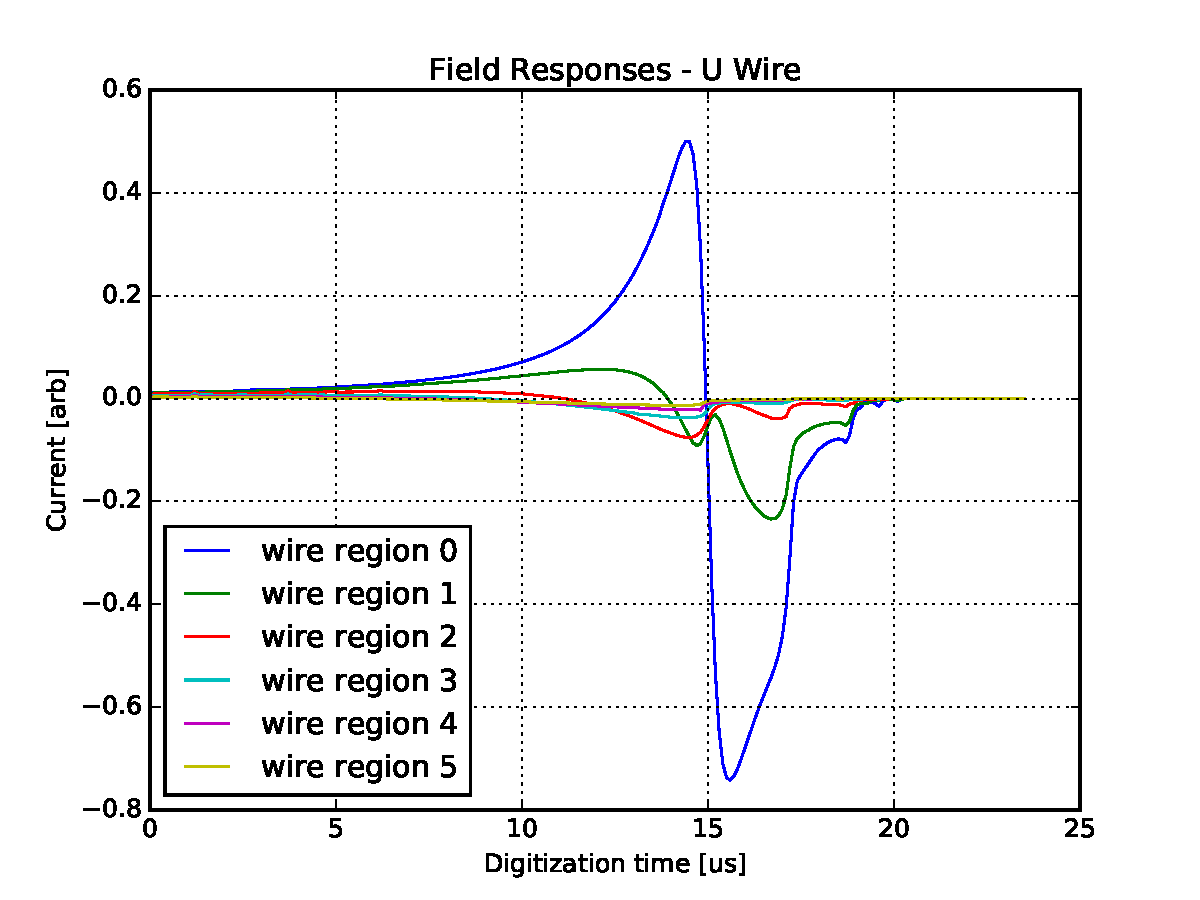
\includegraphics[height=5cm,clip,trim=0 0cm 0 0cm]{current-responses.pdf}
  \end{center}
  \begin{itemize}
  \item Response on wire 0 due to charge drifting in its region
  \item Wire regions 1-5 progressively further.
  \item Wire regions 6-9 not shown.
  \end{itemize}
\end{frame}

\section{Todo}

\begin{frame}
  \frametitle{Work Still To Do}
  \begin{itemize}
  \item Finish with $\mu$Boone-like wires.
  \item Start on DUNE-like wires.
    \begin{itemize}
    \item Approximately 30 unique wires compared to $\mu$B's 3!
    \end{itemize}
  \item Look at design improvements of novel wire plane ideas.
  \end{itemize}
\end{frame}

\section{}
\begin{frame}
  \frametitle{Software}
  \begin{itemize}
  \item BEM++ for the heavy lifting: \\
    \url{http://www.bempp.org/}
  \item ParaView for visualization: \\
    \url{http://www.paraview.org/}
  \item LARF to glue it all together: \\
    \url{https://github.com/brettviren/larf}
  \end{itemize}
  
\end{frame}

\end{document}
%%% Local Variables:
%%% mode: latex
%%% TeX-master: t
%%% End:
